\documentclass{article}
\usepackage[T1]{fontenc}
\usepackage{lmodern}
\usepackage[utf8]{inputenc}
\usepackage[british]{babel}
\usepackage{geometry}
\usepackage{color}
\usepackage{amsthm}
\usepackage{amsmath,amssymb}
\usepackage{graphicx}
\usepackage{mathtools}
\usepackage{listings}
\usepackage{newlfont}
\usepackage{tikz-cd}
\usepackage{faktor}

\newcommand{\numberset}{\mathbb}
\newcommand{\N}{\numberset{N}}
\newcommand{\Z}{\numberset{Z}}
\newcommand{\R}{\numberset{R}}
\newcommand{\Q}{\numberset{Q}}
\newcommand{\C}{\numberset{C}}
\newcommand{\K}{\numberset{K}}
\newcommand{\F}{\numberset{F}}
\newcommand{\n}{\mathcal{N}}
\newcommand{\aid}{\mathfrak{a}}
\newcommand{\bid}{\mathfrak{b}}
\newcommand{\pid}{\mathfrak{p}}
\newcommand{\qid}{\mathfrak{q}}
\newcommand{\mi}{\mathfrak{m}}
\newcommand{\I}{\mathbb{I}}
\newcommand{\V}{\mathbb{V}}

\DeclareMathOperator{\Ima}{Im}
\DeclareMathOperator{\sgn}{sgn}

\newcommand{\exercise}[1]{\noindent {\bf Exercise #1}}

\begin{document}

\title{Algebraic Topology 1 - Assignment 4}

\author{M. Durante, 2303760, Leiden University\\T.A.H.A Quemener, 2304252, Leiden University}

\maketitle


\exercise{1}

We will exibit a retract $G$ from $M$ to a subspace homeomorphic to $S^1$:

\begin{align*}
		G:M\times I & \rightarrow M \\
		([x,y],t) & \rightarrow [x,(1-t)y]
\end{align*}

This function is continuous, with $G(-,0)=Id_M$ and $\Ima(G(-,1))=\{[x,y]\in M\ |\ y=0\}$.

Now, to show that this subspace is homeomorphic to $S^1$, we will consider the following maps:

\begin{align*}
		g:\Ima(G(-,1)) & \rightarrow S^1 \\
		[x,0] & \rightarrow e^{i\pi x} \\
		f:S^1 & \rightarrow \Ima(G(-,1)) \\
		z & \rightarrow [\arg(z)/\pi,0]
\end{align*}

They are both continuous and inverse to each other, thus they are homeomorphisms. We have proved that there is a deformation retract of $M$ homeomorphic to $S^1$.

Since homology groups are invariant under homotopy equivalence, we get that:
$$H_n(M,A)\cong\begin{cases}
		A\textit{ if } n\leq 1 \\
		0\textit{ otherwise}
\end{cases}$$

Let $M_1\sqcup M_2=\{(i,[x,y])\ |\ i\in\{1,2\},\ [x,y]\in M\}$, $F=(M_1\sqcup M_2)/\sim$. Let $U,V\subset F$ be the sets obtained by removing from $F$ respectively $\{[j,[x,y]]\in F\ |\ j=1, y=0\}$ and $\{[j,[x,y]]\in F\ |\ j=2, y=0\}$, which are closed. Clearly, $U\cup V=F$. By the following retraction, $U$ is homotopy equivalent to $S^1$ and by a similar one the same goes for $V$.

\begin{align*}
		G':U\times I & \rightarrow U \\
		([j,[x,y]],t) & \rightarrow\begin{cases}
				[1,[x,(1-2t)y+2t\sgn(y)]]\textit{ if } j=1,\ t\in[0,1/2] \\
				[2,[x,y]]\textit{ if } j=2,\ t\in[0,1/2] \\
				[2,[x,2(1-t)\sgn(y)]]\textit{ if } j=1,\ t\in[1/2,1] \\
				[2,[x,2(1-t)y]]\textit{ if } j=2,\ t\in[1/2,1]
		\end{cases}
\end{align*}

Again, this is continuous, $G(-,0)=Id_U$ and $\Ima(G(-,1))=\{[j,[x,y]]\in F\ |\j=1,\ y=0\}$. Furthermore, the following homeomorphisms show that $\Ima(G(-,1))\cong S^1$:

\begin{align*}
		g:\Ima(G(-,1)) & \rightarrow S^1 \\
		[x,0] & \rightarrow e^{i\pi x} \\
		f:S^1 & \rightarrow \Ima(G(-,1)) \\
		z & \rightarrow [\arg(z)/\pi,0]
\end{align*}

Now, $U\cap V=\{[j,[x,y]]\in F\ |\ y\neq 0\}$. By the following retraction, we shall show that it is homotopy equivalent to $\partial M$:
\begin{align*}
		G'':(U\cap V)\times I & \rightarrow U\cap V \\
		([j,[x,y]],t) & \rightarrow [j,[x,(1-t)y+t\sgn(y)]]
\end{align*}

As always, $G''$ is continuous, $G(-,0)=Id_{U\cap V}$ and $\Ima(G(-,1))=\{[j,[x,y]]\in F\ |\ y=\pm 1\}$.

Now, let's define the desired homeomorphism ($j$ doesn't distinguish points in $\Ima(G(-,1))$ because of the equivalence relation):
\begin{align*}
		g':\Ima(G(-,1)) & \rightarrow\partial M \\
		[j,[x,y]] & \rightarrow [x,y] \\
		f':\partial M & \rightarrow \Ima(G(-,1)) \\
		[x,y] & \rightarrow [j,[x,y]]
\end{align*}

These are continuous maps inverse to each other, thus we have proved that $U\cap V$ is homotopy equivalent to $\partial M$.

Furthermore, by the following homeomorphisms, $\partial M\cong S^1$:
\begin{align*}
		g'':\Ima(G(-,1)) & \rightarrow\partial M \\
		[x,y] & \rightarrow ye^{i\pi x} \\
		f'':\partial M & \rightarrow \Ima(G(-,1)) \\
		z & \rightarrow [\arg(z)/\pi,y]\textit{ where } y=1\textit{ if } \Ima(z)\geq 0,\ y=-1\textit{ otherwise}
\end{align*}

Now, we shall make use of the Mayer-Vietoris (exact!) sequence:
$$\ldots\rightarrow H_n(U\cap V,A)\rightarrow H_n(U,A)\oplus H_n(V,A)\rightarrow H_n(F,A)\rightarrow H_{n-1}(U\cap V,A)\rightarrow\ldots$$

This sequence, taking into account the previously shown isomorphisms, becomes:
$$\ldots\rightarrow H_n(\partial M,A)\rightarrow H_n(S^1,A)\oplus H_n(S^1,A)\rightarrow H_n(F,A)\rightarrow H_{n-1}(\partial M,A)\rightarrow\ldots$$

Let's look at the section of sequence with $n\geq 3$. There, it is:
$$\ldots\rightarrow 0\rightarrow 0\rightarrow H_n(F,A)\rightarrow 0\rightarrow\ldots$$

By exactness, $H_n(F,A)\cong 0$.

Now, we will focus on $n<3$.

\begin{align*}
		0 &\rightarrow H_2(U\cap V,A)\rightarrow H_2(U,A)\oplus H_2(V,A)\rightarrow H_2(F,A)\rightarrow \\
		& \rightarrow H_1(U\cap V,A)\rightarrow H_1(U,A)\oplus H_1(V,A)\rightarrow H_1(F,A)\rightarrow \\
		& \rightarrow H_0(U\cap V,A)\rightarrow H_0(U,A)\oplus H_0(V,A)\rightarrow H_0(F,A)\rightarrow 0
\end{align*}

Which is:
\begin{align*}
		0 &\rightarrow 0\rightarrow 0\rightarrow H_2(F,A)\rightarrow \\
		& \rightarrow A\rightarrow A^2\rightarrow H_1(F,A)\rightarrow \\
		& \rightarrow A\rightarrow A^2\rightarrow H_0(F,A)\rightarrow 0
\end{align*}

Being $F$ path connected ($U$ and $V$ are because of the homotopy equivalence and their intersection is not empty), $H_0(F,A)\cong A$. Since the homomorphism $A\rightarrow A^2$ only involves path-connected components, it can be described as $a\mapsto (a,a)$, hence it is injective.

Now we get this:$$0\rightarrow H_2(F,A)\rightarrow A\rightarrow A^2\rightarrow H_1(F,A)\rightarrow 0$$

The problem now is finding out where the $1$-cicles in $C[\partial M,A]$ are mapped by the obvious inclusion maps into $C[S^1,A]\oplus C[S^1,A]$. We see that these are functions which are non-zero only on loops in $\partial M$ (i.e. in the intersection $U\cap V$) and these loops are generated up to homotopy by a fundamental loop which wraps $\partial M$ once (look at $\pi_1(S^1)$). However, to do so, in the retraction of $U$ to $S^1$ we showed earlier, this loop has to wrap $S^1$ twice, hence $i_*^U(a)=2a$ and by a similar reasoning, because of the orientation, $j_*^V(a)=-2a$. By exactness, $H_1(F,A)\cong A^2/<(2a,-2a)\ |\ a\in A>\cong A^2/<(2a,2a)\ |\ a\in A>\cong A\oplus A/2A$, and $H_2(F,A)\cong 0$.

$(e)$ This surface is the Klein bottle.


~\\
\exercise{2}

$(a)$ I will prove by induction that $|\beta_n(v_0,\ldots,v_n)|=(n+1)!$.

For $n=0$, it is obvious. Let it be true for $n-1$, $n>0$. By definition, being $b$ the barycenter,$$\beta_{n}(v_0,\ldots,v_n)=\{(w_0,\ldots,w_{n-1},b)\ |\ (w_0,\ldots,w_{n-1})\in\beta_{n-1}(\partial(v_0,\ldots,v_n)\}$$

Now, it all comes down to computing $|\beta_{n-1}(\partial(v_0,\ldots,v_n))|$ since the elements in $\beta_{n}(v_0,\ldots,v_n)$ are created by adding $b$ as the $n$th vertex, and so there is a bijection.

We know that $\beta_{n-1}(\partial(v_0,\ldots,v_n))=\cup_{i=0}^n\beta_{n-1}(v_0,\ldots,v_{i-1},v_{i+1},\ldots,v_n)$. By inductive hypothesis, being the sets in the following union disjoint, $|\cup_{i=0}^n\beta_{n-1}(v_0,\ldots,v_{i-1},v_{i+1},\ldots,v_n)|=\sum_{i=0}^n|\beta_{n-1}(v_0,\ldots,v_{i-1},v_{i+1},\ldots,v_n)|=(n+1)n!=(n+1)!$, which concludes the proof.

Now, we prove that two $n$-simpleces in the subdivision are internally disjoint. Indeed, consider $[v_1,\ldots,v_n,b]$ and $[v_0,v_2,\ldots,v_n,b]$ (the same proof, modulo computations, holds for every other choice of $n$-simpleces). The elements in the intersection satisfy the following:$$\sum_{i=1}^n t_iv_i+bt=\sum_{j=0,j\neq 1}^n t'_jv_j+t'b$$

Which translates to:$$\sum_{i=1}^n (t_i+\frac{t}{n+1})v_i+\frac{t}{n+1}v_0=\sum_{j=0,j\neq 1}^n (t'_j+\frac{t'}{n+1})v_j+\frac{t'}{n+1}v_1$$

Since the $v_i$ are linearly independent, we get a system of equations:
\begin{align*}
		t_i+\frac{t}{n+1}-t'_i-\frac{t'}{n+1} & =0\ \ \forall i\in\{2,\ldots,n\} \\
		t_1+\frac{t}{n+1}-\frac{t'}{n+1} & =0 \\
		\frac{t}{n+1}-t'_0-\frac{t'}{n+1} & =0 \\
		\sum_{i=1}^n t_i+t=\sum_{j=0,j\neq 1}^n t'_j+t' & =1,\ \ t,t_i,t',t'_j\geq 0
\end{align*}

This is a system of $n+3$ equations in $2n+2$ variables. By noticing that all of the rows are linearly independent (ignoring for a moment the fact that $t,t_i,t',t'_j\geq 0$), we find a $(n-1)$-dimensional vector space, hence the intersection among the two happens along the boundary (it is a $(n-1)$-simplex) and they do not share interior points.

It follows that, if two $n$-simpleces in the first subdivision are distinct, the simpleces created from their subdivisions will be distinct as well, since these are contained in the simplex they were created from and have non-empty intersection with the interior (i.e. they are not contained in the boundary of the simplex). By a similar argument, this holds for every iteration of the subdivision process.

Since at each iteration $m$ the simpleces in the subdivision will generate distinct simpleces, we get that $|K^{m+1}|=(n+1)!|K^m|$. Given that $|K^0|=|\{\Delta^n\}|$, $|K^m|=((n+1)!)^m$.

$(b)$ To prove the bijection, we only have to compute the number of such chains (we have already shown that $|K^1|=(n+1)!$).

Such a chain can be seen as a finite succession of vertices: indeed, at each step a vertex is removed from the set, thus we may identify $F_i$ with $x\in F_i\setminus F_{i-1}$. Given that the process terminates after $n$ steps, i.e. when only one element remains, and at each step the possible choices diminish by 1, starting from $n+1$, we get that the number of possible successions (and hence chains), is exactly $(n+1)((n+1)-1)\cdots ((n+1)-(n-1))=(n+1)n\cdots 2=(n+1)!$.

$(c)$ We will apply Apollonius' Theorem to find a triangle having in its own barycentric subdivision a similar triangle. We know that the barycenter divides a median in two parts, whose lengths have ratio 2:1, the longer one being the one with a vertex corresponding to one of the triangle.

We get the following system of equations:
\begin{align*}
		(\frac{c'}{b'})^2 & =(\frac{c}{b})^2 \\
		(\frac{a'}{b'})^2 & =(\frac{a}{b})^2 \\
		b'^2 & =\frac{c^2}{4} \\
		c'^2 & =(\frac{1}{3})^2\frac{a^2+b^2-\frac{c^2}{2}}{2} \\
		a'^2 & =(\frac{1}{3})^2\frac{b^2+c^2-\frac{a^2}{2}}{2} \\
		a & =1
\end{align*}

Computing, we find that such a triangle (up to scaling) has sides of length length $a=1,b=\sqrt{2}/2,c=\sqrt{3}/2$.

Let's check that what we have found has the desired properties.

\begin{figure}
		  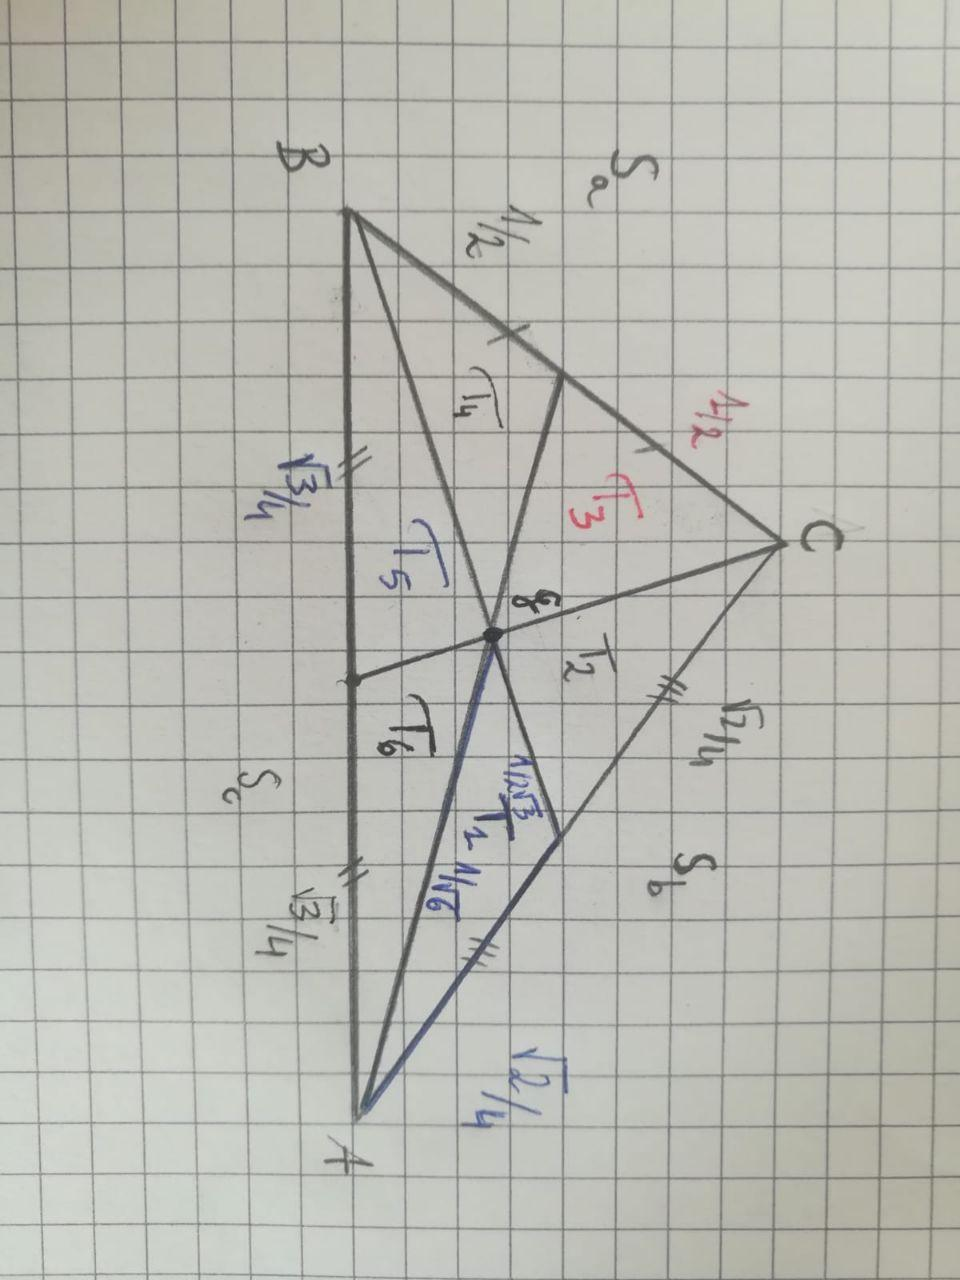
\includegraphics[width=6cm]{pic1ass4at1.jpg}
		  \caption{Barycentric subdivision of the triangle}
\end{figure}

We may compute the lengths of the medians through the parallelogram law: $m_i=\frac{1}{2}\sqrt{2(s_j^2+s_k^2)-s_i^2}$ is the length of the median bisecting the side $s_i$.

Now, we get that:
\begin{align*}
		m_a=\frac{1}{2}\sqrt{2(\frac{1}{2}+\frac{3}{4})-1}=\frac{\sqrt{6}}{4} \\
		m_b=\frac{1}{2}\sqrt{2(1+\frac{3}{4})-\frac{1}{2}}=\frac{\sqrt{3}}{2} \\
		m_c=\frac{1}{2}\sqrt{2(1+\frac{1}{4})-\frac{3}{4}}=\frac{\sqrt{3}}{4}
\end{align*}

Here, $a',b'$ and $c'$ are respectively $\overrightarrow{A\mathcal{G}},\overrightarrow{\mathcal{G}B'}$ and $\overrightarrow{AB'}$.

We have that $\mathcal{T}_{1}$ is similar to the original triangle with a ration of $\frac{1}{\sqrt{6}}$. Indeed, we have $\overrightarrow{A\mathcal{G}}=(\frac{2}{3})\overrightarrow{AA'}$, where $A'$ is the other extremity of the median of length $m_{a}=\frac{\sqrt{6}}{4}$, hence $||\overrightarrow{A\mathcal{G}}||=(\frac{2}{3})(\frac{\sqrt{6}}{4})=\frac{1}{\sqrt6}=1(\frac{1}{\sqrt6})$\\
In a same fashion we also have that $||\overrightarrow{\mathcal{G} B'}||=(\frac{1}{3})(\frac{\sqrt{3}}{2})=(\frac{1}{\sqrt{12}})=(\frac{1}{\sqrt{6}})(\frac{\sqrt{2}}{2})$
And finally, we have that $|| \overrightarrow{A\mathcal{B'}}||=\frac{1}{2}(\frac{\sqrt2}{2})=\frac{1}{\sqrt6}(\frac{\sqrt3}{2})$.

Clearly, we may find a 2-affine simplex in $\R^2$ whose sides would have length $1,\sqrt{2}/2$ and $\sqrt{3}{2}$, hence we are done.

\end{document}
